% Logo de FisGraf: una curva ajustada sobre mediciones con barras de error.
% Se convierte a PNG e ICO con `cargo run --example generar_logo`.
\documentclass[tikz,border=0pt]{standalone}
\begin{document}
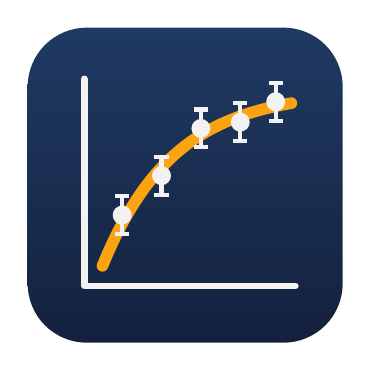
\begin{tikzpicture}
  \definecolor{fondo}{HTML}{14213D}
  \definecolor{fondo2}{HTML}{1F3A63}
  \definecolor{curva}{HTML}{FCA311}
  \definecolor{punto}{HTML}{F2F2F2}
  % Fondo: cuadrado redondeado con degradado suave.
  \shade[top color=fondo2, bottom color=fondo, rounded corners=0.75cm] (0,0) rectangle (4,4);
  % Ejes.
  \draw[punto, line width=2.4pt, line cap=round, line join=round] (0.72,3.35) -- (0.72,0.72) -- (3.4,0.72);
  % Curva ajustada.
  \draw[curva, line width=4.2pt, line cap=round]
    plot[smooth, domain=0.95:3.35, samples=50] (\x, {0.85 + 2.35*(1 - exp(-(\x - 0.9)*1.1))});
  % Mediciones con barras de error y topes.
  \foreach \x/\y in {1.2/1.62, 1.7/2.12, 2.2/2.72, 2.7/2.80, 3.15/3.06} {
    \draw[punto, line width=1.5pt] (\x, \y - 0.24) -- (\x, \y + 0.24);
    \draw[punto, line width=1.5pt] (\x - 0.09, \y - 0.24) -- (\x + 0.09, \y - 0.24);
    \draw[punto, line width=1.5pt] (\x - 0.09, \y + 0.24) -- (\x + 0.09, \y + 0.24);
    \fill[punto] (\x, \y) circle (0.12);
  }
\end{tikzpicture}
\end{document}
